\documentclass[]{finalproject}
\captionsetup{labelfont={bf}}
\usepackage{graphicx,subfigure}
\def\textsubscript#1{\ensuremath{_{\mbox{\textscale{.6}{#1}}}}}
\usepackage{color}
\newcommand\tab[1][1cm]{\hspace*{#1}}
\usepackage{graphicx}
\graphicspath{ {C:\Users\muhammed\Pictures\ } }
\usepackage{verbatim}

% Title (and subtitle) of the project

\title{Decomposition Algorithms}
%\subtitle{(Decomposion Algorithms)}

% Group members for the final project (comment out the unnecessary entries)
\begin{groupmembers}
\studentA{Muhammet}{USLU}{}
\studentB{Mao}{(Yen)}{PO}
\end{groupmembers}

\abstract {
This project outlines the factorization of matrices with the six most widely used decomposition algorithms according to \cite{algorithms}
}


\begin{document}
\maketitle

%%%%%%%%%%%%%%%%%%%%%%%%%
\section{Introduction} \label{introduction}

\begin{flushleft}

We use the terms decomposition and factorization interchangeably to mean writing a matrix as a product of two or more other simpler matrices, generally with some defined properties (such as lower/upper triangular). \newline
The underlying principle of the decomposition approach to matrix computation is that to construct computational platforms from which a variety of problems can be solved.
The article deals primarily with dense matrix computations. Although the decomposition approach has greatly influenced iterative and direct methods for sparse matrices. \newline \newline
\textbf{Benefits of the decomposition approach :} 
\begin{flushleft}
• Matrix decomposition solves not one but many problems. \newline
• Matrix decomposition, which is generally expensive to compute, can be reused to solve new problems involving the original matrix.\newline
• The decomposition approach facilitates rounding-error analysis.\newline
\end{flushleft}
We will focus on six most widely used  algorithms namely; Cholesky, LU, Spectral, SVD, Schur, QR. For sure these are not the only used methods.
\newline
\end{flushleft}

\section{Cholesky} \label{cholesky}

\begin{flushleft}

If a matrix M is symmetric ( $\mathbf{M}^\intercal$ = M ), positive semi-definite ( all eigenvalues are non-negative ) or a complex Hermitian matrix ( M = $\overline{M}^\intercal$ ) then we can use $\mathbf{LL}^\intercal$ factorization such that L is a lower triangular matrix. \cite{cholesky} \\
$\linebreak $
\tab   
M = L * $\mathbf{L}^\intercal$ $\qquad$ $\longrightarrow$ $\qquad$
$\begin{bmatrix} 
m_{1,1} & m_{1,2} & m_{1,3}\\
m_{2,1} & m_{2,2} & m_{2,3}\\
m_{3,1} & m_{3,2} & m_{3,3}
\end{bmatrix}$
$\qquad$ = $\qquad$
$\begin{bmatrix}
l_{1,1} & 0 & 0\\
l_{2,1} & l_{2,2} & 0\\
l_{3,1} & l_{3,2} & l_{3,3}
\end{bmatrix}$ *
$\begin{bmatrix}
l_{1,1} & l_{1,2} & l_{1,3}\\
0 & l_{2,2} & l_{2,3}\\
0 & 0 & l_{3,3}
\end{bmatrix}$
$\newline$ $\newline$ $\newline$ 
\tab \tab \tab  = $\qquad$
$\begin{bmatrix}
l_{1,1}^{2} & l_{1,1}*l_{2,1} & l_{1,1}*l_{3,1}\\
l_{2,1}*l_{1,1} & l_{2,1}^{2}+l_{2,2}^{2} & l_{2,1}*l_{3,1}+l_{2,2}*l_{3,2}\\
l_{3,1}*l_{1,1} & l_{3,1}*l_{2,1}+l_{3,2}*l_{2,2} & l_{3,1}^{2}+l_{3,2}^{2}+l_{3,3}^{2}
\end{bmatrix}$
$\newline$ $\newline$
So we can generalize the formulas for higher dimensional matrices...$\newline$ $\newline$
$l_{i,i}$ = $\sqrt{m_{i,i} - \sum_{j=1}^{i-1} l_{i,j}^{2}}$ $\quad$ for i = 1,2,... n
and $\quad$ %for the elements below the diagonal
for i > j $\quad$ $l_{i,j} = \frac{m_{i,j} - \sum_{k = 1}^{j-1}  l_{i,k} * l_{j,k}} {l_{j,j}}$ with i = 1,2,... n and j =  1,2,... i-1
$\newline$

\begin{comment}
\textbf{Numerical Example:}  $\newline$ $\newline$ Consider 3x3 matrix $\qquad$ 
$\begin{bmatrix}
4 & 2 & 6\\
2 & 2 & 5\\
6 & 5 & 22
\end{bmatrix}$ $\qquad$ executing the formulas above gives us the following entries of lower triangular matrix L  $\newline$  
$l_{1,1}$ = $\sqrt{4}$ = 2 $\quad$ $l_{2,1}$ = $\dfrac{2}{2}$ = 1 $\quad$ $l_{3,1}$ = $\dfrac{6}{2}$ = 3 $\quad$
$l_{2,2}$ = $\sqrt{2-1}$ = 1 $\quad$ $l_{3,2}$ = $\dfrac{5-3*1}{1}$ = 1 $\quad$ $l_{3,3}$ = $\sqrt{22-9-4}$ = 3 $\newline$ $\newline$
so L = 
$\begin{bmatrix}
2 & 0 & 0\\
1 & 1 & 0\\
3 & 2 & 3
\end{bmatrix}$
\end{comment}

\textbf{ The Computational Cost:} 
Computing diagonal element $l_{i,i}$ requires \begin{flushleft}
• i subtractions\\
• i - 1 multiplications, and\\
• one square root,
\end{flushleft}
which adds up to 2i operations so overall diagonal element calculation costs us $\sum_{i = 1}^{n} {2i}$ = 2 $\dfrac{n*(n+1)}{2} = n^{2}+n $ $\newline$

On the other hand $l_{i,j}$ requires \begin{flushleft}
• j subtractions\\
• j - 1 multiplications, and\\
• one division,
\end{flushleft} so totally 2j operations, then for n dimensional matrix it will require 
$\sum_{i = 1}^{n} {\sum_{j = 1}^{i - 1} {2j}} = \sum_{i = 1}^{n} {2\frac{(i-1)*i}{2}} = \frac{n^{3}}{3} - \frac{n}{3}  $   floating-point operations. $\newline$

Finally summing up those two costs results by the domination of $\frac{n^{3}}{3} $ Flops $\newline$ $\newline$
Note : if M is very sparse, most of elements of the matrix are zero , L is often (but not always) sparse then if L is sparse, the cost of the factorization is much less than $\frac{n^{3}}{3}$   $\newline$
Cholesky factorization is numerically stable; instability is characterized by significant changes in the predicted dynamical behaviour induced by only small changes in the specification of the system. \newline \newline


\textbf{Application:} Quantum Chemistry; cholesky decomposition of the two-electron integral matrix \cite{cholesky_application} \newline
\begin{comment}
Chemists must seek methods that combine the sparsity for large systems and exploit the linear dependence in the product space of atomic orbitals.\newline
The Cholesky decomposition of the atomic orbital (AO) two-electron integrals may be written as; \newline
$ (\mu \nu \vert \lambda \sigma) = \sum_{K=1}^{M} A_{\mu \nu}^{K} A_{\lambda \sigma}^{K}$ where Greek letters denote atomic orbitals and M is the number of Cholesky vectors A. \newline
Advantage in this application: \newline
Accuracy of representation of the exact two-electron repulsion integrals(ERIs) is controlled only by a single parameter, the so-called Cholesky Decomposition threshold $ \delta $. By construction, it provides an upper bound to the absolute difference between an exact ERI and its approximated value so by using the Cholesky Factorization the error introduced in entries in AO matrix can be seen as same order as in results. 
The disadvantage is the total price in the number of operations. \newline \newline
\end{comment}

%$\newline$ $\newline$ $\newline$ $\newline$ $\newline$ $\newline$ $\newline$ $\newline$ $\newline$ $\newline$ $\newline$ $\newline$

\end{flushleft}



\section{LU} \label{lu}
\begin{flushleft}
An invertible matrix M has an LU decomposition , L is an lower-triangular matrix with all diagonal entries equal to 1 and U is an upper-triangular matrix,  provided that all its leading sub-matrices are non-singular (with non-zero determinants). \linebreak
The $k^{th}$ leading sub-matrix of M is denoted $M_{k}$ and is the k×k matrix found by looking only at the top k rows and leftmost k columns. \linebreak
Thanks to Pivoting (so called row interchange); it is always possible to re-order the rows of an invertible matrix so that all of the sub-matrices have non-zero determinants. That is why this decomposition is also called LUP factorization, P is the permutation matrix. \cite{lu}
\linebreak 
Let us assume there is no pivoting so the P = I \linebreak \linebreak
M = L * U * P $\qquad$ $\longrightarrow$ $\qquad$
$\begin{bmatrix} 
m_{1,1} & m_{1,2} & m_{1,3}\\
m_{2,1} & m_{2,2} & m_{2,3}\\
m_{3,1} & m_{3,2} & m_{3,3}
\end{bmatrix}$
$\quad$ = $\quad$
$\begin{bmatrix}
1 & 0 & 0\\
l_{2,1} & 1 & 0\\
l_{3,1} & l_{3,2} & 1
\end{bmatrix}$ *
$\begin{bmatrix}
u_{1,1} & u_{1,2} & u_{1,3}\\
0 & u_{2,2} & u_{2,3}\\
0 & 0 & u_{3,3}
\end{bmatrix}$
*
$\begin{bmatrix}
1 & 0 & 0\\
0 & 1 & 0\\
0 & 0 & 1
\end{bmatrix}$

$\newline$ $\newline$ $\newline$ 
\tab \tab \tab  = $\qquad$
$\begin{bmatrix}
u_{1,1} & u_{1,2} & u_{1,3}\\
l_{2,1}*u_{1,1} & l_{2,1}*u_{1,2} + u_{2,2} & l_{2,1}*u_{1,3} + u_{2,3}\\
l_{3,1}*u_{1,1} & l_{3,1}*u_{1,2} + l_{3,2}*u_{2,2} & l_{3,1}*u_{1,3}+l_{3,2}*u_{2,3}+u_{3,3}
\end{bmatrix}$
\newline \newline \newline
Generalized formulas : \newline
$u_{ij} = m_{ij} - \sum_{k=1}^{i-1}  u_{kj} * l_{ik}$  $\qquad for \quad j = 1,2,... n \quad i = 1,2,...j+1 \quad k = 1,2,...i$ 
\newline
$l_{ij} = \frac{1}{u_{jj}} * (m_{ij} - \sum_{k=1}^{j-1} u_{kj} * l_{ik} \quad and \quad l_{j,j} = 1 
\qquad for \quad j = 1,2,... n \quad i = j,j+1,...n \quad k = 1,2,...j$ \linebreak The total cost is $\dfrac{2}{3}n^{3}$ Flop
\newline

\begin{comment}
\textbf{Numerical Example:} Effect of Rounding Error with a different Pivoting configuration $\newline$ $\newline$ Consider Mx=b in matrix form; $\quad$ 
$\begin{bmatrix}
10^{-5} & 1 \\
1 & 1 
\end{bmatrix}$
$\begin{bmatrix}
x_{1} \\
x_{2}
\end{bmatrix}$ \quad = \quad 
$\begin{bmatrix}
1 \\
0
\end{bmatrix}$,
Exact solutions are $x_{1} = \frac{-1}{1-10^{-5}}$ and $x_{2} = \frac{1}{1-10^{-5}}$ \quad Let us solve the equations using LU factorization, rounding intermediate results to 4 significant decimal digits.\newline
we will do this for the two possible permutation matrices:\newline
\qquad $P_{1} = \begin{bmatrix}
1 & 0 \\
0 & 1 
\end{bmatrix}$ \quad  or 
\quad $P_{2} = \begin{bmatrix}
0 & 1 \\
1 & 0 
\end{bmatrix}$ \newline
With first choice (no pivoting $P_{1}$); 
$\begin{bmatrix}
10^{-5} & 0 \\
1 & 1 
\end{bmatrix}$ = 
$\begin{bmatrix}
1 & 0 \\
10^{5} & 1 
\end{bmatrix}$ * $\begin{bmatrix}
10^{-5} & 1 \\
0 & 1-10^{5}\longmapsto-10^{5}  
\end{bmatrix}$ after forward and back substitution $x_{1} = 0, x_{2} = 1$ so error in $x_{1}$ is 100$ \% $ \newline

With second choice (Pivot interchange $P_{2}$); 
$\begin{bmatrix}
10^{-5} & 0 \\
1 & 1 
\end{bmatrix}$ = 
$\begin{bmatrix}
1 & 0 \\
10^{-5} & 1 
\end{bmatrix}$ * $\begin{bmatrix}
1 & 1 \\
0 & 1-10^{-5}\longmapsto 1 
\end{bmatrix}$ after forward and back substitution $x_{1} = -1, x_{2} = 1$ so error in $x_{1}$, $x_{2}$ is about $10^{-5}$\newline
\end{comment}



Some features of LU Decomposition:
\begin{flushleft}
• For some choices of P, small rounding errors in the algorithm cause very
large errors in the solution (numerical instability).\\
• when P permutes the largest element (absolute value) of first column of M to the 1,1-position.
\end{flushleft}


\textbf{Application:} Power Engineering; Power Flow Computation \cite{lu_application} \newline
\begin{comment}Power flow calculation is needed for analysis of a power system network to model the steady state of the system. Between end points there are sets of nodes (Buses) and every node has the following electrical properties; \newline
active power $ P_{i}(x) $ and reactive power  $ Q_{i}(x) $ such that we can represent the apparent power $ S_{i}(x) $ = $ P_{i}(x) $ + J$ Q_{i}(x) $ difference between all the apparent power from every nodes and predicted values of them are collected in a matrix (this matrix is generally quite sparse) \newline
To analyse the system dynamics such as, resistance, inductance... we need to decompose this matrix. \newline
Since they use specifically configured hardware (FPGA) to solve the sparse matrix they get roughly $ n^{1.4} $ Flop so LU De composition can outperform with sparse matrix and special hardware. 
\end{comment}


%$\newline$ $\newline$ $\newline$ $\newline$ $\newline$ $\newline$ $\newline$ $\newline$ $\newline$ $\newline$ $\newline$ $\newline$ $\newline$ $\newline$ $\newline$ $\newline$ $\newline$

\end{flushleft}
\

\section{SPECTRAL} \label{spectral}
\begin{flushleft}
The Spectral Decomposition recasts a matrix in terms of its eigenvalues and eigenvectors. This representation
turns out to be enormously useful. \linebreak
Each symmetric M (nxn) matrix can be written as $PDP^{-1}$ or $PDP^{T}$, where D is $diag(\lambda_{1}, ... ,\lambda_{n})$ , $\lambda_{i}$ is the corresponding eigenvalue and where P (Jordan canonical form)is an orthogonal matrix, ($v_{1}, .... ,v_{n}$) , consisting of the orthonormal eigenvectors $v_{i}$. One important side note is orthogonal matrices have unit norm. \cite{spectral}
\linebreak 
\linebreak \linebreak
M = P * D * $P^{T}$ $\qquad$ $\longrightarrow$ $\qquad$
$\begin{bmatrix} 
m_{1,1} & m_{1,2} & m_{1,3}\\
m_{2,1} & m_{2,2} & m_{2,3}\\
m_{3,1} & m_{3,2} & m_{3,3}
\end{bmatrix}$
$\quad$ = $\quad$
$\begin{bmatrix} 
\uparrow & \uparrow & \uparrow\\
v_{1} & v_{2} & v_{3}\\
\downarrow & \downarrow & \downarrow
\end{bmatrix}$ *
$\begin{bmatrix}
\lambda_{1} & 0 & 0\\
0 & \lambda_{2} & 0\\
0 & 0 & \lambda_{3}
\end{bmatrix}$
*
$\begin{bmatrix}
\leftarrow & v_{1} & \rightarrow\\
\leftarrow & v_{2} & \rightarrow\\
\leftarrow & v_{3} & \rightarrow
\end{bmatrix}$ 
$\newline$

Generalized formula : \newline

M = $\sum_{i=1}^{n}  \lambda_{i} * v_{i}*v_{i}^{T} \qquad for \quad i = 1,2,... n $
$\newline$  $\newline$ 
Some Usefull features of Spectral Factorization:\newline
$\ast$ The Jordan decomposition gives a representation of a symmetric matrix in terms of eigenvalues and eigenvectors.

$\ast$ The eigenvectors belonging to the largest eigenvalues indicate the ``main direction'' of the data.

$\ast$ The Jordan decomposition allows one to easily compute the power of a symmetric matrix $M^{\alpha} = P * D^{\alpha} *P^{T}$ 
$\newline$ 

\begin{comment}
\textbf{Numerical Example:} $\newline$ $\newline$ 
Let M = 
$\begin{bmatrix} 
1 & 1 & 3\\
1 & 3 & 1\\
3 & 1 & 1
\end{bmatrix}$
Characteristic polynomial of M is $p_{M}$($\lambda$) = det(M - $\lambda$ I) so the eigenvalues are -2, 2, 5 and the corresponding
eigenspaces are all one dimensional, spanned by the eigenvectors;\newline
$v_{1} = 
\begin{bmatrix} 
1 \\
0 \\
-1 
\end{bmatrix}$  \qquad
$v_{2} = 
\begin{bmatrix} 
1 \\
-2 \\
1 
\end{bmatrix}$ \qquad
$v_{3} = 
\begin{bmatrix} 
1 \\
1 \\
1 
\end{bmatrix}$  After scaling the eigenvectors results getting the orthogonal matrix \newline \newline
\newline
P = $\begin{bmatrix} 
\frac{v_{1}}{\Vert v_{1} \Vert} & \frac{v_{2}}{\Vert v_{2} \Vert} & \frac{v_{3}}{\Vert v_{3} \Vert} 
\end{bmatrix}$ = 
$\begin{bmatrix} 
\dfrac{1}{\sqrt{2}} & \dfrac{1}{\sqrt{6}} & \dfrac{1}{\sqrt{3}}\\
0 & \dfrac{2}{\sqrt{6}} & \dfrac{1}{\sqrt{3}}\\
\dfrac{-1}{\sqrt{2}} & \dfrac{1}{\sqrt{6}} & \dfrac{1}{\sqrt{3}}
\end{bmatrix}$ and the eigenvalues are found D = 
$\begin{bmatrix} 
-2 & 0 & 0\\
0 & 2 & 0\\
0 & 0 & 5
\end{bmatrix}$\newline \newline
\end{comment}
Note : The Spectral Decomposition is a special kind of Eigenvalue Decomposition in which the matrix P is orthogonal which means that the eigenvectors are orthonormal. 
An Eigenvalue Decomposition is a special kind of Jordan Decomposition in which the "Jordan form" matrix is diagonal. \cite{jordan} \newline
\textbf{Application:} LTI Systems with a state space representation. \cite{jordan_application} \newline

\begin{comment}
Matrix exponential, $ e^{tM} $,where M is n×n, is a state transition matrix for LTI systems with a state space representation. The matrix exponential was defined as follows: \newline
$ e^{tM} = I + \sum_{k=1}^{\infty} \dfrac{t^{k}M^{k}}{k!} = I + tM + \dfrac{t^{2}M^{2}}{2!} + .... + \dfrac{t^{k}M^{k}}{k!} + ... $ \newline
When the n × n matrix M is diagonalizable, $ e^{tM} $ becomes particularly easy to evaluate, then we will use the features of Spectral Decomposition;\newline
$ (M)^{k} = (P * D * P^{-1})^{k} $ =  $ P * D^{k} * P^{-1} $  substituting into the series expansion; 
$ e^{tM} = P( I+ tD +  \dfrac{t^{2}D^{2}}{2!} + .... + \dfrac{t^{k}D^{k}}{k!} + ... )P^{-1} $ Now using the definition of the function $ e^{x} $ as power series: $ e^{x} = \sum_{k=0}^{\infty} \dfrac{x^{k}}{k!} $ we have that
 $ e^{tM} = P
 \begin{bmatrix} 
e^{t\lambda_{1}} & & &  \\
 &e^{t\lambda_{2}} & & \\
 & &\ddots & \\
& & &&e^{t\lambda_{n}}
\end{bmatrix} P^{-1}$
\end{comment}


%$\newline$ $\newline$ $\newline$ $\newline$ $\newline$ $\newline$ $\newline$ $\newline$ $\newline$ $\newline$ $\newline$ $\newline$ $\newline$ $\newline$ $\newline$ $\newline$ $\newline$

\end{flushleft}


\section{SVD} \label{svd}
\begin{flushleft}
Let m and n be arbitrary ; we don’t not require $m \geqslant n$. Given M $\epsilon$ $C^{mxn}$, not necessarily of full rank, a SVD of M is a factorization \newline \newline
$ M = U \Sigma V^{*} $ $\qquad$ $\longrightarrow$ $\qquad$
$\begin{bmatrix} 
\uparrow &  & \uparrow\\
m_{1} & ... & m_{n}\\
\downarrow & & \downarrow
\end{bmatrix}$
$\quad$ = $\quad$
$\begin{bmatrix} 
\uparrow &  & \uparrow\\
u_{1} & ... & u_{n}\\
\downarrow & & \downarrow
\end{bmatrix}$
$\begin{bmatrix}
\sigma_{1} &  & \\
 & \sigma_{2} & \\
 & & \sigma_{p}
\end{bmatrix}$
$\begin{bmatrix} 
\uparrow &  & \uparrow\\
v_{1} & ... & v_{n}\\
\downarrow & & \downarrow
\end{bmatrix} ^{-T}$
\newline \newline \newline
with $U \epsilon C^{mxn}$ unitary, $V \epsilon C^{nxn}$ unitary, $\Sigma \epsilon R^{mxn}$ diagonal. \linebreak
In addition, it is assumed that the diagonal entries $\sigma_{j}$ of $\Sigma$ are non-negative and in non-increasing order; 
 that is, $\sigma_{1} \geqslant \sigma_{2} \geqslant . . .  \geqslant \sigma_{p} \geqslant 0$ where p = min(m,n) The diagonal matrix $\Sigma$ has the same shape as M even when M is not square, but U and V are always square unitary matrices. \cite{svd} \newline \newline
\textbf{Different between Eigenvalue(Spectral) Decomposition and SVD:}\newline
$ A \epsilon C^{mxn}, B \epsilon C^{mxm} $ \newline
$ B = P D P^{-1} $ ; P is collection of eigenvectors of B ,$ D $ is diagonal matrix with eigenvalue \newline
$ A = U \Sigma V^{*}$ ; u is left eigenvector in m dimension, v is right eigenvector in n dimension , $ \Sigma $ is diagonal matrix with singular value.\newline
 $AA^{*} = U\Sigma V^{*}(U \Sigma V^{*})^{T} = U\Sigma V^{*}(V \Sigma U^{*}) =  U\Sigma(\Sigma U^{*}) = U\Sigma^{2} U^{*}$ U is eigenvector of $AA^{*}$, $\Sigma^{2} $  is eigenvalue of $AA^{*}$ \newline \newline
 

\textbf{Application:} Principal Components Analysis \cite{svd} \newline

\begin{comment}
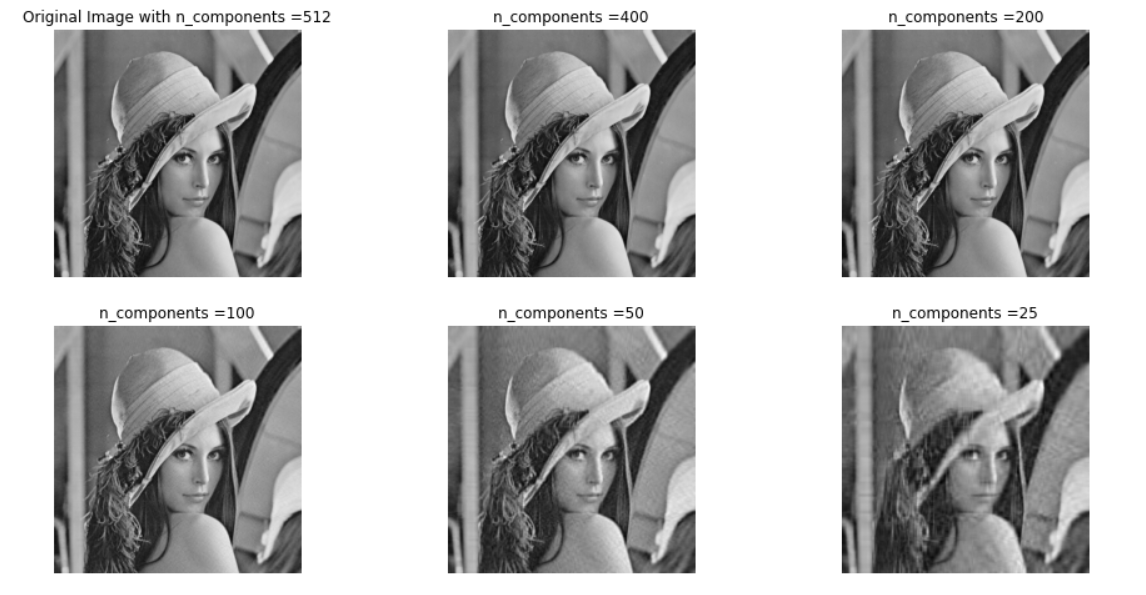
\includegraphics[width=1\linewidth]{svd_app.png}
\begin{center} Image Compression \end{center} 

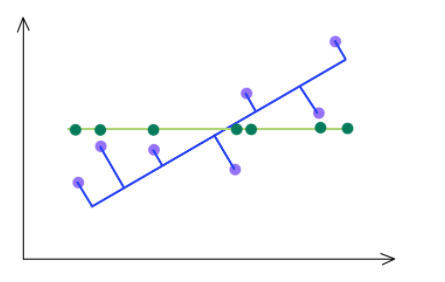
\includegraphics[width=1\linewidth]{svd_app1.png}
\begin{center} Principal Components Analysis \end{center} 
 
\textbf{Numerical Example:}  $\newline$ $\newline$ 
Let M = 
$\begin{bmatrix} 
3 & 4\\
0 & 5
\end{bmatrix}$ \quad so $MM^{T}$ = 
$\begin{bmatrix} 
25 & 20\\
20 & 25
\end{bmatrix}$ \newline
The eigenvectors of $MM^{T}$ solve the following equation ($MM^{T}$ - $\lambda$ I)x = 0 \newline
Find the eigenvalue $ \lambda $; det($MM^{T}$ - $\lambda$ I)= 0
The eigenvalues will be  $ \lambda_{1} = 45$ and $\lambda_{2} = 5$ \newline
In order to find the eigenvectors we can write det($MM^{T}$ - $\lambda$ I) = 0 as follows;\newline
$\begin{bmatrix} 
25- \lambda_{i} & 20\\
20 & 25 - \lambda_{i}
\end{bmatrix}$
$\begin{bmatrix} 
x_{1} \\
x_{2}
\end{bmatrix}$ = 0 for i = 1,2 since we have two eigenvalues. Then $ u_{1} $ = $\begin{bmatrix} 
\frac{1}{\sqrt{2}} \\
\frac{1}{\sqrt{2}}
\end{bmatrix}$ and $ u_{1} $ = $\begin{bmatrix} 
\frac{1}{\sqrt{2}} \\
\frac{-1}{\sqrt{2}}
\end{bmatrix}$ \newline
Left orthogonal matrix U = [$u_{1}$ $u_{2}$] = 
$\begin{bmatrix} 
\frac{1}{\sqrt{2}} & \frac{1}{\sqrt{2}}\\
\frac{1}{\sqrt{2}} & \frac{-
1}{\sqrt{2}}
\end{bmatrix}$ \newline
In order to find V and $ \Sigma $ matrices we will calculate the eigenvectors of $M^{*}$M; for any real symmetric matrix M, its eigenvalues are the same as that of $ M^{*} $ witch means $(M M^{*})^{*} $ = $M^{*}$M\newline
$M^{T}$M = $\begin{bmatrix} 
9 & 12\\
12 & 41
\end{bmatrix} \longrightarrow $  so as before $ \lambda_{1} $ = 45 and $ \lambda_{2} $ = 5 however the eigenvectors should change. \newline \newline
$ v_{1} $ = $\begin{bmatrix} 
\frac{1}{\sqrt{10}} \\
\frac{3}{\sqrt{10}}
\end{bmatrix}$ and $ v_{1} $ = $\begin{bmatrix} 
\frac{-3}{\sqrt{10}} \\
\frac{1}{\sqrt{10}}
\end{bmatrix}$ so V = [$v_{1}$ $v_{2}$] = 
$\begin{bmatrix} 
\frac{1}{\sqrt{10}} & \frac{-3}{\sqrt{10}}\\
\frac{3}{\sqrt{10}} & \frac{1}{\sqrt{10}}
\end{bmatrix}$ finally $ \Sigma $ =
$\begin{bmatrix} 
\sigma_{1} & 0\\
0 & \sigma_{2}
\end{bmatrix}$  =
$\begin{bmatrix} 
\sqrt{\lambda_{1}} & 0\\
0 & \sqrt{\lambda_{2}}
\end{bmatrix}$ =
$\begin{bmatrix} 
3\sqrt{5} & 0\\
0 & \sqrt{5}
\end{bmatrix}$ \newline \newline 
The composed form : 
$\begin{bmatrix} 
3 & 4\\
0 & 5
\end{bmatrix}$ = 
$\begin{bmatrix} 
\frac{1}{\sqrt{2}} & \frac{1}{\sqrt{2}}\\
\frac{1}{\sqrt{2}} & \frac{-1}{\sqrt{2}}
\end{bmatrix}$ 
$\begin{bmatrix} 
3\sqrt{5} & 0\\
0 & \sqrt{5}
\end{bmatrix}$
$\begin{bmatrix} 
\frac{1}{\sqrt{10}} & \frac{-3}{\sqrt{10}}\\
\frac{3}{\sqrt{10}} & \frac{1}{\sqrt{10}}
\end{bmatrix}$ 

\end{comment}
%$\newline$ $\newline$ $\newline$ $\newline$ $\newline$ $\newline$ $\newline$ $\newline$ $\newline$ $\newline$ $\newline$ $\newline$ $\newline$ $\newline$ $\newline$ $\newline$ $\newline$

\end{flushleft}


\section{SCHUR} \label{schur}
\begin{flushleft}
Consider this matrix: \newline \newline
A = $\begin{bmatrix} 
13 & 8 & 8 \\
-1 & 7 & -2 \\
-1 & -2 & 7
\end{bmatrix} $  How do we get $ A^{60} $ ? \newline \newline
Easiest way is using A = $P D P^{-1} $ \qquad $ A^{60}$ = $P D^{60} P^{-1}$ (eigenvalue decomposition), in fact that does not work for this matrix. However we can do something almost as good
For any given matrix, the Schur decomposition allows to find another matrix that is similar to the given one and is upper triangular. \newline \newline
A = UT$U^{*}$ \qquad $ U_{2}U_{1}AU_{1}U_{2} = \begin{bmatrix} 
\lambda_{1} & . & .\\
0 & \lambda_{2} & .\\
0 & 0 & \lambda_{3}
\end{bmatrix} = U^{*}TU$ \newline \newline
where T is upper triangular, with the eigenvalues of A on its diagonal, and U was a unitary matrix. \newline
The Schur decomposition is not unique
we choose an eigenvalue arbitrarily; as a consequence, there are different possible orderings of the eigenvalues of A on the main diagonal of T. \newline
More in general, if \qquad $ U^{*}AU = T $ \qquad is a Schur decomposition of A, we can take any unitary matrix Q such that $ Q^{*}TQ $ \newline
is upper triangular, and use it to construct another Schur decomposition $ (UQ)^{*}A(UQ) = Q^{*}TQ $ \cite{schur} \newline
 
\begin{comment} 
\textbf{Numerical Example:}  $\newline$ $\newline$ 
A =  $\begin{bmatrix} 
13 & 8 & 8 \\
-1 & 7 & -2 \\
-1 & -2 & 7
\end{bmatrix} $ First, we want an eigenvector of A. Start with find the eigenvalues so $ det(A - \lambda I) = 0 $ \newline
The eigenvalues are $ \lambda = 9 $ then we can find an eigenvector:  $ det(A - \lambda I)\begin{bmatrix} 
x \\
y  \\
z 
\end{bmatrix} = $  x + 2y + 2z = 0, one of solutions can be (2, -2, 1) normalized $u_{1}=\dfrac{1}{3}[2, -2, 1]$ \newline
We want an orthonormal basis for this space. To do so, we first find a basis, and then use Gram-Schmidt orthogonal. We can see that (0, 1, -1) is in our space (x + 2y + 2z = 0), \newline \newline
$ u_{2 } $= (0, 1, -1) - proj((0, 1, -1)  onto (2, -2, 1))  \newline \newline
$(0, 1, -1) - \frac{(0, 1, -1)*(2, -2, 1)}{\Vert (2,-2,1)\Vert ^{2}}(2,-2,1)$ = $ (0, 1, -1) - \frac{-3}{9}(2, -2, 1) $ = $(\frac{6}{9}, \frac{3}{9}, \frac{-6}{9})$ if we normalize then $ u_{2} = \frac{1}{3}[2, 1, -2] $ \newline

We now need to extend this to a basis for all of $C^{3}$: to do this, we simply take some vector not in the span of these two vectors, like (0, 0, 1), and perform Gram-Schmidt on this third vector. \newline
$ u_{3}$ = (0, 0, -1) - proj((0, 0, -1)  onto (2, -2, 1)) - proj((0, 0, -1)  onto (2, 1, -2)) \newline
= (0, 0, -1)- $ \frac{1}{9} $ (2, -2, 1) - $\frac{-2}{9}$ (2, 1, -2) = $\frac{4}{9}$ (1, 2, 2)  normalized get 
$u_{3} = \frac{1}{3}$ [1, 2, 2] \newline \newline
U = $ \frac{1}{3} \begin{bmatrix} 
2 & 2 & 1 \\
-2 & 1 & 2 \\
1 & -2 & 2
\end{bmatrix} $ \qquad T =  $ U^{*}AU $ = $ \frac{1}{3} \begin{bmatrix} 
2 & -2 & 1 \\
2 & 1 & -2 \\
1 & 2 & 2
\end{bmatrix} 
\begin{bmatrix} 
13 & 8 & 8 \\
-1 & -7 & -2 \\
-1 & -2 & 7
\end{bmatrix}
\frac{1}{3}
\begin{bmatrix} 
2 & 2 & 1 \\
-2 & 1 & 2 \\
1 & -2 & 2
\end{bmatrix} $ \newline \newline \newline
T = $\frac{1}{9}
\begin{bmatrix} 
81 & 0 & 81 \\
0 & 81 & 81 \\
0 & 0 & 81
\end{bmatrix} $ = 
$\begin{bmatrix} 
9 & 0 & 9 \\
0 & 9 & 9 \\
0 & 0 & 9
\end{bmatrix} $ so then $A^{60}$ = 
$\frac{1}{3} \begin{bmatrix} 
2 & 2 & 1 \\
-2 & 1 & 2 \\
1 & -2 & 2
\end{bmatrix} 
\begin{bmatrix} 
9 & 0 & 9 \\
0 & 9 & 9 \\
0 & 0 & 9
\end{bmatrix}^{60}
\frac{1}{3} \begin{bmatrix} 
2 & -2 & 1 \\
2 & 1 & -2 \\
1 & 2 & 2
\end{bmatrix} $
\end{comment}

%$\newline$ $\newline$ $\newline$ $\newline$ $\newline$ $\newline$ $\newline$ $\newline$ $\newline$ $\newline$ $\newline$ $\newline$ $\newline$ $\newline$ $\newline$ $\newline$ $\newline$

\end{flushleft}


\section{QR} \label{qr}
\begin{flushleft}
QR factorization is often used to solve the linear least squares problem.
Assume that M $\epsilon C^{mxn} (m \geq n)$ has full rank n. 
\linebreak 
M = Q * R $\qquad$ $\longrightarrow$ $\qquad$
$\begin{bmatrix} 
\uparrow &  & \uparrow\\
m_{1} & ... & m_{n}\\
\downarrow & & \downarrow
\end{bmatrix}$
$\quad$ = $\quad$
$\begin{bmatrix} 
\uparrow &  & \uparrow\\
q_{1} & ... & q_{n}\\
\downarrow & & \downarrow
\end{bmatrix}$ *
$\begin{bmatrix} 
r_{1,1} & \cdots & r_{1,n}\\
 & \ddots & \vdots\\
 &  & r_{n,n}
\end{bmatrix}$ \linebreak \newline
Written out these equations as linear combination of $m_{1}, m_{2}, ... m_{n}$  and take the form; \newline
$m_{1} = r_{11}*q_{1} \newline
m_{2} = r_{12}*q_{1} + r_{22}*q_{2} \newline
. \newline
. \newline
. \newline
m_{n} = r_{1n}*q_{1} + r_{2n}*q_{2} +...+r_{nn}*q_{n} $
\newline
As a matrix formula, we have M = $\hat{Q} * \hat{R}$ called reduced QR Factorization \newline
Q-factor:
\begin{flushleft}
• Q is mxn matrix with orthogonal columns ($Q^{T}*Q = I$) \newline
• If M ıs a square (m=n) matrix, then Q is orthogonal ($Q^{T}*Q = Q*Q^{T} =I$)
\end{flushleft}  

R-factor:
\begin{flushleft}
• Q is nxn upper triangular matrix with non zero diagonal elements ($r_{kk} \not= 0 $) \newline
• R is non-singular (diagonal elements are non-zero)
\end{flushleft}
\textbf{Full QR Factorization}: \cite{qr} \newline
QR factorization of a matrix M $\epsilon C^{mxn}$, appending an additional m-n orthogonal to columns so $\hat{Q}$ becomes an mxn matrix. \newline
\textbf{2 Group:} :  \newline
Orthogonal triangularization-Householder  $ Q_{n}...Q_{2}Q_{1}A = R $ \newline
Triangular orthogonalization- Gram-Schmidt $ AR_{1}R_{2}...R_{n} = Q $ \newline \newline

\textbf{Algorithms for QR factorization} \newline
Modified Gram-Schmidt algorithm: complexity for mxn dimensional matrix; $\sum_{k=1}^{n} (4m-1)(k-1)-3m) \quad = \quad  (4m-1)\frac{n(n-1)}{2}+3mn$
\begin{center}
  = $2mn^{2}$ Flops
\end{center}
Householder Algorithm:\newline
$\sum_{k=1}^{n} 4(m-k+1)(n-k+1) \quad = \quad  \int_{0}^{n} 4(m-t)(n-t) \,dt $
\begin{center}
  = $2mn^{2} - \dfrac{2}{3}n^{3}$ Flops
\end{center}
SVD $\sim 2mn^{2} + 11n^{3} $ flops \newline 
Normal equation $\sim mn^{2} + \dfrac{1}{3}n^{3} $ flops \newline

\begin{comment}
\textbf{Numerical Example :} $\newline$ $\newline$ 
A = $\begin{bmatrix}
1 & 2 \\
0 & 1 \\
1 & 0
\end{bmatrix}$ we take first column of A as $ V_{1} $ = $\begin{bmatrix}
1\\
0\\
1
\end{bmatrix}$ We take norm of $ V_{1} $ as $ r_{1,1} $ \newline \newline

$ r_{1,1} $ = $\Vert  V_{1} \Vert$ = $\sqrt{2}$ normalized $ V_{1} $  get $ q_{1} $ = ${\begin{bmatrix}
\dfrac{1}{\sqrt{2}} \\ 
0 \\ 
\dfrac{1}{\sqrt{2}}
\end{bmatrix} } $ and 
$ r_{1,2} $ = $ q_{1}^{*} V_{2} $ = $\begin{bmatrix}
\dfrac{1}{\sqrt{2}} & 0 & \dfrac{1}{\sqrt{2}}
\end{bmatrix} \begin{bmatrix}
2 \\ 
1 \\ 
0
\end{bmatrix}$ = $\sqrt{2}$ \newline

$ V_{2}  =  V_{1} - r_{1,2}q_{1} $ = $\begin{bmatrix}
1 \\ 
1 \\ 
-1
\end{bmatrix}$ and normalized $ V_{2} $  get $ q_{2} $ = $\begin{bmatrix}
\dfrac{1}{\sqrt{3}} \\ 
\dfrac{1}{\sqrt{3}} \\ 
\dfrac{-1}{\sqrt{3}}
\end{bmatrix}$  
Finally A = $\begin{bmatrix}
\dfrac{1}{\sqrt{2}} & \dfrac{1}{\sqrt{3}} \\ 
0 & \dfrac{1}{\sqrt{3}}\\ 
\dfrac{1}{\sqrt{2}} & \dfrac{-1}{\sqrt{3}}
\end{bmatrix} 
\begin{bmatrix}
\sqrt{2} & \sqrt{2} \\ 
0 & \sqrt{3}
\end{bmatrix} $ \newline \newline \newline \newline

A = $\begin{bmatrix}
12 & -51 & 4 \\
6 & 167 & -68  \\
-4 & 24 & -41 
\end{bmatrix}$ \newline \newline
compute reflector that maps first column of A to multiple of e1: \newline
$ w_{1} = q_{1}- \Vert a_{1} \Vert e1  $ = $\begin{bmatrix}
12 \\ 
6 \\ 
-4
\end{bmatrix} -14
\begin{bmatrix}
1 \\ 
0 \\ 
0
\end{bmatrix} $ = $\begin{bmatrix}
-2 \\ 
6 \\ 
4
\end{bmatrix}$ then $ V_{1} = \dfrac{w_{1}}{\Vert w_{1} \Vert} $ = $ \dfrac{1}{14} \begin{bmatrix}
-1 \\ 
3 \\ 
-2
\end{bmatrix} $ \newline \newline

$Q_{1} = I - 2V_{1}V_{1}^{T} = \begin{bmatrix}
\dfrac{6}{7} & \dfrac{3}{7} & \dfrac{-2}{7}\\ \\
\dfrac{3}{7} & \dfrac{-2}{7} & \dfrac{6}{7}  \\ \\
\dfrac{-2}{7} & \dfrac{6}{7} & \dfrac{3}{7} 
\end{bmatrix} $ so $Q_{1}A = 
\begin{bmatrix}
14 & 21 & 14 \\ \\
0 & -49 & -14  \\ \\
0 & 168 & -77 
\end{bmatrix} $ so we are close to a upper triangular matrix. We \newline only need to zero the (3, 2) entry. \newline
Take the (1, 1) minor, and then apply the process again; \newline
$ A^{'} = \begin{bmatrix}
-49 & -14  \\ 
168 & -77
\end{bmatrix} $ By the same method as above $ w_{2} = q_{1}- \Vert a_{1} \Vert e1  $ = $\begin{bmatrix}
-224 \\ 
168 
\end{bmatrix} $ and $Q_{2} = I - 2V_{2}V_{2}^{T} = \begin{bmatrix}
\frac{-7}{25} & \frac{24}{25}\\
\frac{24}{25} & \frac{7}{25}
\end{bmatrix} $ \newline We expand to 3*3 matrix \newline

$Q_{2} = \begin{bmatrix}
1 & 0 & 0 \\
0 & \frac{-7}{25} & \frac{24}{25}  \\
0 & \frac{24}{25} & \frac{7}{25}
\end{bmatrix} $  so finally $ R = Q_{2}Q_{1}A = Q^{T}A = 
\begin{bmatrix}
1 & 0 & 0 \\
0 & \frac{-7}{25} & \frac{24}{25}  \\
0 & \frac{24}{25} & \frac{7}{25}
\end{bmatrix}
\begin{bmatrix}
14 & 21 & 14 \\ 
0 & -49 & -14  \\ 
0 & 168 & -77 
\end{bmatrix} =
\begin{bmatrix}
14 & 21 & -14 \\ 
0 & -49 & -70  \\ 
0 & 0 & 35 
\end{bmatrix} $
\end{comment}


%$\newline$ $\newline$ $\newline$ $\newline$ $\newline$ $\newline$ 
\clearpage
\end{flushleft}

\section{Results} \label{results}
\begin{flushleft}
All results can be reproduced from our project in \href{https://github.com/uslumt/Efficient_Computational_Algorithms}{\fcolorbox{green}{white}{\textbf{GitHub Repository}}}.
\begin{figure}[!h]
\centering     %%% not \center
\subfigure[]{\label{fig:a}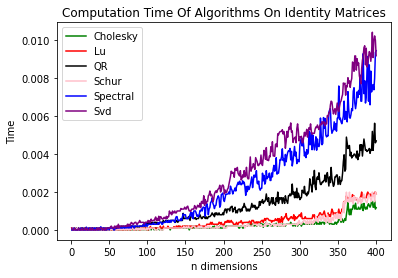
\includegraphics[width=0.31\linewidth]{Computation_time_identity.png}}
\subfigure[]{\label{fig:b}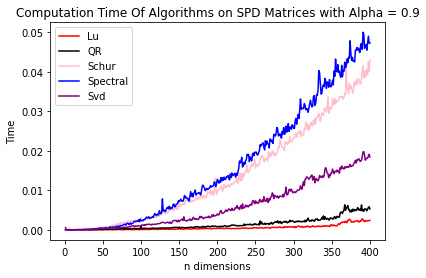
\includegraphics[width=0.33\linewidth]{Computation_time_alpha_0.9.png}}
\subfigure[]{\label{fig:b}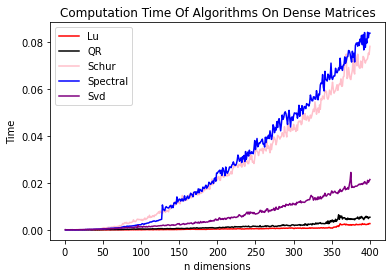
\includegraphics[width=0.3\linewidth]{Computation_time_dense.png}}
\caption{Illustrates the computation time of the algorithms versus increasing dimension of matrices. Since identity matrix has the eigenvalues on its diagonal it helps Schur and Spectral to compute fast than SVD however if there are other entries as it can be seen in (b) (c) those algorithms struggle to calculate eigenvalues and eigenvectors. In theorem SVD has the highest $2*m*n^{2}$ + $11*n^{3}$ flops and Cholesky has the lowest $mn^{2} + \frac{1}{3}n^{3}$ flops.
As the result SVD also cost the highest time on compute and Cholesky is on the bottom of graph which cost the least time Specifically (a) shows that how all algorithms perform on identity matrix, naturally Symmetric Positive Definite, and (b) outlines 5 algorithms on SPD dataset however we had to leave out Cholesky because empirically since \href{https://scikit-learn.org/stable/modules/generated/sklearn.datasets.make_sparse_spd_matrix.html#sklearn.datasets.make_sparse_spd_matrix}{\textbf{Sklearn}} uses randomization, Finally (c) illustrates the algorithms perform on dense dataset. }
\end{figure}


\begin{figure}[!h]
\centering   
\subfigure[]{\label{fig:a}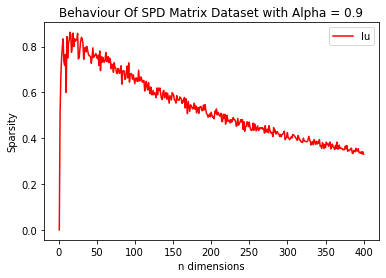
\includegraphics[width=0.31\linewidth]{Behaviour_spd_alpha_0.9.png}}
\subfigure[]{\label{fig:b}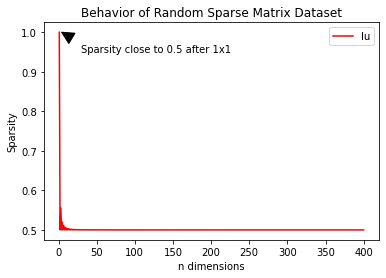
\includegraphics[width=0.31\linewidth]{Behaviour_random_sparsity_0.5.png}}
\subfigure[]{\label{fig:b}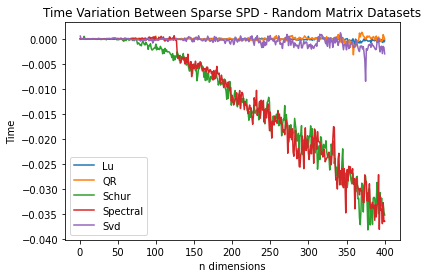
\includegraphics[width=0.34\linewidth]{SparseSPD-DenseRandom.png}}
\caption{From (a) and (b) plots it can be seen that how the datasets behave when different sparsity rates are passed. As it is shown there is a non linearity situation in Symmetric Positive Definite matrix as the dimension increases. In (c) the main take away is how diagonalization effects on SPD and dense matrix; as the dimension of matrix increases SVD, QR, LU, decompositions are hardly effective however with Spectral and Schur, SPD matrix is decomposed easier}
\end{figure}


\begin{table}[!h]
\centering
\begin{tabular}{ll}
\textcolor[rgb]{0.141,0.161,0.184}{Algorithm}                    & Outcome                                                 \\
\textcolor[rgb]{0.141,0.161,0.184}{QR-Householder}               & \textcolor[rgb]{0.133,0.133,0.133}{1.000000284809481}   \\
\textcolor[rgb]{0.141,0.161,0.184}{QR-Gram-Schmidt}              & \textcolor[rgb]{0.133,0.133,0.133}{0.981779891867633}   \\
\textcolor[rgb]{0.141,0.161,0.184}{Normal Equation}                     & \textcolor[rgb]{0.133,0.133,0.133}{-0.390537644183687}  \\
\textcolor[rgb]{0.141,0.161,0.184}{Singular Value Decomposition} & \textcolor[rgb]{0.133,0.133,0.133}{1.000000284809170}   \\
\textcolor[rgb]{0.141,0.161,0.184}{LUP}                          & \textcolor[rgb]{0.133,0.133,0.133}{~0.999999951596828} 
\end{tabular}

\caption{Vandermonde Least Squares Problem Results : Thanks to the normalization, it is known that the true value of x (in A*x = b) will equal to 1. This means that all algorithms are accurate, especially SVD, QR-householder and LU with partial pivoting . QR-householder is more stable than QR using Gram-Schmidt that concludes the theorem in \cite{matlab_referece}}
\end{table}

\end{flushleft}
\clearpage

\section{Conclusion} \label{conclusion}
\begin{flushleft}
Given the guidance of the original paper on which this report is based on, we were able to explore the decompositional approach. \newline
We confirm that the introduction of matrix decomposition into scientific computations brought convenient and sustainable platforms. \newline
We have experienced how to do literature review and scripting pseudo codes to actual program via using open source tools.
During the project it was quite easy to reconstruct or import modules for algorithms however while researching for dataset, especially Symmetric Positive Definite matrices, we could not really find a high quality open source dataset in Python Programming Language. \newline
To sum up we have learned more insights and thought our fellow students the matrix factorization algorithms. \newline

As a future work it can be possible to extend our project with some embedded factorization algorithms on different datasets.


\end{flushleft}

\section{Work Division} \label{work}
\begin{flushleft}
Muhammet USLU : I have reviewed research papers, state of the art applications and solved numerical examples on Cholesky, LU and Spectral Decompositions.
I set up all the Jupyter Notebook structure to make Mao`s test runs convenient, tidy and document the used algorithms to more readable.
As we stated in this report some algorithms requires special type of matrices I did research for datasets. I have written LaTex format of the final report.\newline

Mao PO : I was responsible for QR, Schur and Singular Value Decomposition. I wrote Matlab script for vandermonde matrix to test algorithms stability by solving Least Squares problems. I compared different matrices and algorithms from Muhammet`s work and visualize by plotting graphics. I handle errors in Python program.

\end{flushleft}
\clearpage

\bibliography{references}
\bibliographystyle{unsrt}
\clearpage
\end{document}
